% insert figures into the article.
% 'h' to put the figure at the right place.
% 't' to put the figure at the top of the page.
% 'b' to put the figure at the bottom of the page.
% 'p' to create a blank page for the figure.
\begin{figure}[h!]
    \centering
    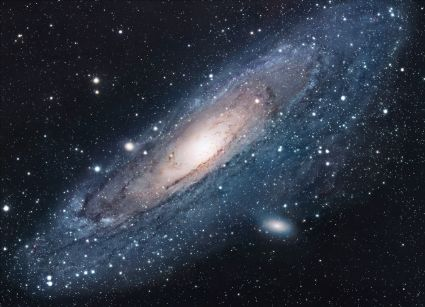
\includegraphics[height=5cm ,width=8cm,angle=0]{universe.jpg}
    \caption{The Universe}
    \label{fig:universe}
\end{figure}

% insert multiple figures in a group into the article.
\begin{figure}[t!]
    \centering
    \subfigure[1st] {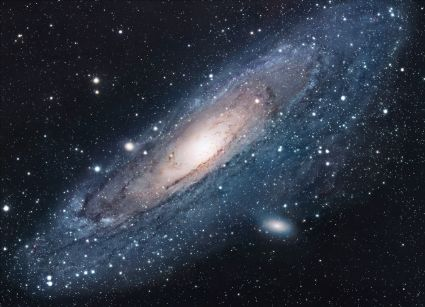
\includegraphics[height=2in,width=2in,angle=-90]{universe.jpg}}
    \subfigure[2nd] {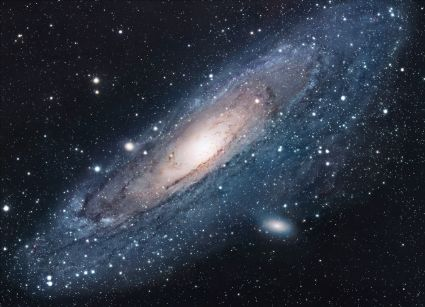
\includegraphics[height=2in,width=2in,angle=-90]{universe.jpg}}
    \subfigure[3rd] {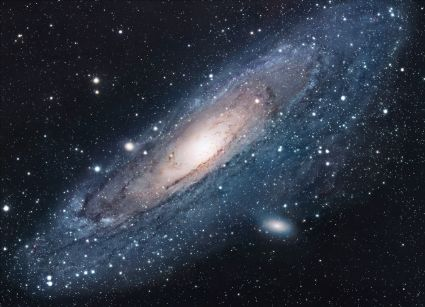
\includegraphics[height=2in,width=2in,angle=-90]{universe.jpg}}
    \caption{The Universe}
    \label{fig:universe2}
\end{figure}